%
% Supplement for Reproducibility manuscript
%
% arara: make
% arara: pdflatex
% arara: bibtex
% arara: pdflatex
% arara: pdflatex
% arara: clean: {files: [SI.aux, SI.bbl, SI.blg, SI.log, acs-SI.bib, SI.fls]}
%


\documentclass[journal=jctcce,manuscript=suppinfo]{achemso}

\usepackage[T1]{fontenc}
\usepackage{graphicx}
\usepackage{amsmath,amssymb,mathrsfs}
\usepackage{xr}
\usepackage{booktabs}
\usepackage{xcolor}
\usepackage{siunitx}
\usepackage{easy-todo}
\usepackage{footref}

\externaldocument[R-]{reprod}

\sisetup{
  separate-uncertainty = true
}

\renewcommand{\footnoterule}{}
\newcommand{\hred}[1]{\textcolor{red}{#1}}


\title{Reproducing Relative Alchemical Free Energies of Hydration}

\author{Hannes H. Loeffler}
\affiliation[Scientific Computing Department, STFC]{Science \&
  Technology Facilities Council, Daresbury, Warrington, WA4 4AD,
  United Kingdom}
\email{Hannes.Loeffler@stfc.ac.uk} \phone{+44 1925 603367}

\author{Stefano Bosisio}
\affiliation[University of Edinburgh]{EaStCHEM School of Chemistry,
  University of Edinburgh, David Brewster Road, Edinburgh EH9 3FJ, UK}

\author{Guilherme Duarte Ramos Matos}
\affiliation[University of California, Irvine]{Department of
  Chemistry, University of California, Irvine}

\author{Donghyuk Suh}
\affiliation[University of Chicago]{University of Chicago}

\author{Julien Michel}
\affiliation[University of Edinburgh]{EaStCHEM School of Chemistry,
  University of Edinburgh, David Brewster Road, Edinburgh EH9 3FJ, UK}

\author{David L. Mobley}
\affiliation[University of California, Irvine]{Departments of
  Pharmaceutical Sciences and Chemistry, University of California,
  Irvine}

\author{Benoit Roux}
\affiliation[University of Chicago]{University of Chicago}


\keywords{Free Energy, Hydration, Alchemical, Reproducibility}


\begin{document}

\maketitle

% whole table comparing all softwares used in the study
% input files (coordinates and topologies)
% lambda schedules used in the simulations (mdp files?)
% glossary: what do terms used in the main text mean
% . alternatives used by other workers (lots of work! -> worthwhile?)


\section{Softcore Functions}
\label{sec:softcores}

We describe here the softcore functions~\cite{beutler_avoiding_1994,
  zacharias_separationshifted_1994} as implemented in the MD packages
AMBER, CHARMM, Gromacs and Sire.  Both the van der Waals,
$V_{\mathrm{LJ}}$ (Lennard--Jones potential) and the electrostatic
interactions, $V_{\mathrm{Coul}}$ (Coulomb potential) as a function of
the order parameter $\lambda$ are given for the disappearing atoms
only.  For the appearing atoms replace $\lambda$ with $1 - \lambda$
and \emph{vice versa}.  Eq.\ \eqref{eq:general-softcore} is the generalized
form for all codes while the specific distance dependent functions are
outlined in eq.\,\eqref{eq:Sire} for Sire, eq.\,\eqref{eq:Amber} for
AMBER, eq.\,\eqref{eq:Gromacs} for Gromacs and eq.\,\eqref{eq:CHARMM}
for CHARMM.

\begin{equation}
  V = V_{\mathrm{LJ}} + V_{\mathrm{Coul}} =
  4\epsilon_{\mathrm{ij}}(1 - \lambda) \left[ \left(
      \frac{\sigma_{ij}}{\textcolor{red}{r_{\mathrm{LJ}}}}
    \right)^{12} - \left(
      \frac{\sigma_{ij}}{\textcolor{red}{r_{\mathrm{LJ}}}} \right)^{
      6} \right] +
  (1 - \lambda)^{n} \frac{q_{i}q_{j}}
  {4\pi\varepsilon_{0}\textcolor{red}{r_{\mathrm{Coul}}}}
  \label{eq:general-softcore}
\end{equation}

For Sire
\begin{equation}
  \begin{split}
    r_{\mathrm{LJ}} &= (\alpha\sigma_{ij}\lambda + r_{ij}^2)^{\frac{1}{2}} \\
    r_{\mathrm{Coul}} &=  (\lambda + r_{ij}^2)^{\frac{1}{2}}
  \end{split}
  \label{eq:Sire}
\end{equation}

For AMBER
\begin{equation}
  \begin{split}
    r_{\mathrm{LJ}} &= (\alpha \sigma_{ij}^{6} \lambda + % see JCP127, 214108
                         r_{ij}^6)^{\frac{1}{6}} \\
    r_{\mathrm{Coul}} &= (\beta\lambda + r_{ij}^{p})^{\frac{1}{p}} \\
    n &= 1
  \end{split}
  \label{eq:Amber}
\end{equation}

For Gromacs
\begin{equation}
  \begin{split}
    r_{\mathrm{LJ}} &= (\alpha \sigma_{ij}^{w} \lambda^{p} +
    r_{ij}^{w})^{\frac{1}{w}} \\
    &p = 1,2; w = 6,48; \\
    r_{\mathrm{Coul}} &= r_{\mathrm{LJ}} \\
    &\alpha_{\mathrm{Coul}} = 0,\alpha_{\mathrm{LJ}} \\
    n &= 1
  \end{split}
  \label{eq:Gromacs}
\end{equation}

For CHARMM (PSSP), applied to all ``reactant'' and all ``product'' atoms
\begin{equation}
  \begin{split}
    r_{\mathrm{LJ}} &= (\alpha \lambda + r_{ij}^2)^{\frac{1}{2}} \\
    r_{\mathrm{Coul}} &= (\beta\lambda + r_{ij}^{2})^{\frac{1}{2}} \\
    n &= 1
   \end{split}
  \label{eq:CHARMM}
\end{equation}

$r_{\mathrm{vdW}}$, $r_{\mathrm{Coul}}$ and $r_{\mathrm{Coul}}$ (all in red) 
are the distance dependent functions, $\epsilon_{\mathrm{ij}}$ and
$\sigma_{ij}$ are the Lennard-Jones parameters, $q_{i}$ and $q_{j}$
are the charges and $\varepsilon_{0}$ is the vacuum permittivity,
$\alpha$ and $\beta$ are the softcore tuning parameters determining
the softness of the potential, and $r_{ij}$ the distance between
atoms $i$ and $j$.

The exponent $n$ is only used in the Coulomb softcore funtion of Sire.
Gromacs allows additional exponents for $\lambda$ ($p = 1$ or $2$) and
$w$ for the distance dependency with values of either $6$ or $48$.  AMBER 
allows an exponent $p$ (namelist option \textsc{sceeorder}) for the Coulomb 
softcore.  The Coulomb softcore parameter $\alpha_{\mathrm{Coul}}$ in Gromacs 
is the same as for the Lennard--Jones parameter $\alpha_{\mathrm{LJ}}$
unless the Coulomb softcore function is requested not to be used and thus 
$\alpha_{\mathrm{Coul}} = 0$.  The
CHARMM softcore function (PSSP) is applied to \emph{all} atoms in the
perturbed group and not only to dummy atoms as in the other codes.
The perturbed group comprises of all atoms that need to be
transformed, i.e.\ any atom that differs in at least one force field
parameter in the other end state.  ``Dummy'' atom is used here as a
shorthand notation for any atom that appears or disappears during the
course of the transformation.


\section{Split Protocols}
\label{sec:separated}

When the AFE (alchemical free energy) simulation is separated (split) into van
der Waals and Coulomb steps it must be ensured that charges of
vanishing atoms are switched off before the vdW radius is scaled to
zero.  This is to avoid that other atoms e.g.\ from solvent come in
close contact to a charged atom without the associated excluded volume
from the van der Walls term as this could lead to large forces and 
thus instabilities in the integrator.

\begin{figure}[ht]
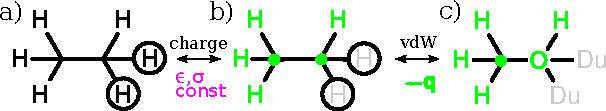
\includegraphics[scale=1.0]{figures/dummies.pdf}
\caption{The mutation of ethane into methanol and explicit topologies
  for three states. a) The two circles denote atoms that have both vdW
  and Coulomb terms switched on with parameters for the respective
  hydrogen atom type.  b) The two hydrogen atoms have their charges
  switched to zero (gray symbols in black circle).  All other charges
  are the ones from the methanol end state c (green) to ensures charge
  neutrality at each step.  VdW parameters are constant in the charge
  transfer step (see annotations in magenta).  c) vdW and Coulomb
  parameters as for methanol while dummy atoms (gray Du) have those
  parameters all set to zero.}
\label{fig:dummies}
\end{figure}

Figure~\ref{fig:dummies} depicts how force field parameters vary for a
transformation carried out in the direction of disappearing atoms.
The mutation is shown with the charge step first followed by the vdW
step but each step can really be run independently.  Please note that
both charge and vdW step would be simulated at a range of individual
$\lambda$s.  Typically the charge transfer is done with linear scaling
while the vdW mutation is done with softcores (see above).  The
transformation is fully symmetrical that is the parameters must be
switched on in opposite order if atoms are to be ``created''.  The
intermediate state b has the vdW parameters from state a but the
charges from state c.

Figure~\ref{fig:dummies} shows how topology files may be created in
cases where the MD software does not allow independent $\lambda$s
for electrostatic and vdW mutations.  With Gromacs, for instance, the
transformation only requires a single topology file with both A and B
states (in single topology fashion, see main text) and a single
simulation control file with separate $\lambda$ vectors for charge and
vdW transformations.  Any intermediate state from
Figure~\ref{fig:dummies} is thus created ``on--the-fly'' i.e.\
implicitly during the simulation run.  With AMBER (up to version 16 as
of this writing), however, three explicit topology files (with sander,
two with pmemd) and two control files would need to be created.  The
state b in Figure~\ref{fig:dummies} would be created from state a with
the charges from state c.  The bonded terms can be combined with
either mutation step or run separately.  For AMBER the easiest way is to
combine vdW with bonded terms because charges are independent of atom
types.

Figure~\ref{fig:dummies2} illustrates explicit topologies for
transformations with both appearing and disappearing atoms in one simulation.  
The principle is essentially the same as in Figure~\ref{fig:dummies}:
charges of dummy atoms must be switched off before vdW parameters are
set to zero to avoid interactions of ``naked'' charge sites with other
atoms possibly leading to very close contact, large energies and
forces, and thus to unstable simulations and/or noisy statistics.
However, charge neutrality at every $\lambda$ step is not supported in
most MD codes i.e.\ the total system charge varies with $\lambda$
unless the charges of \emph{all} atoms are switched off.  Possible
strategies would be to explicitly create topology files for each
intermediate $\lambda$ state and distribute the diminished charges from
the dummy atoms over to the non--dummy atoms.  MD software like CHARMM
allows to do this through internal scripting although this would be just as
extensive as external scripting the aforementioned strategy.

\begin{figure}[ht]
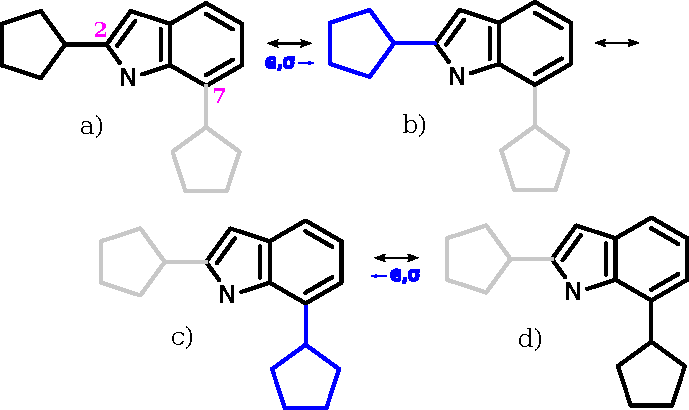
\includegraphics[scale=1.0]{figures/dummies2.pdf}
\caption{Explicit topologies involved in a mutation with both
  appearing and disappearing atoms by example of the cyclopentanyl
  transfer from the 2 position in indole to the 7 position.  Blue
  lines denote atoms which have their charges switched off but with
  vdW parameters from the left (state b) or right (state c). Gray
  lines are dummy atoms with Coulomb and vdW parameters all zero.
  Note, the hydrogen bound to the 2 (state d) and 7 positions (state
  a) can be directly mutated from the respective carbon atom type
  without ring breaking~\cite{doi:10.1021/acs.jcim.5b00057}.}
\label{fig:dummies2}
\end{figure}

With the MD packages tested in this study the number of input files
are as follows.  With Gromacs this can be done with only two topology
and two control files where one charge transfer can be combined with a
vdW on/off step.  Gromacs' $\lambda$ vectors only apply to the
perturbed group as a whole and so it is not possible to define a
$\lambda$ vector for only a subset.  AMBER requires two such files
with sander and three topology/two control files with pmemd for the
three steps charge off, vdw on/off and charge on.  This is possible because
with AMBER a subset of the perturbed group can be chosen to have zero
charges (namelist option \textsc{crgmask}; but AMBER does not have $\lambda$ 
vectors).  CHARMM has scripting facilities that let the user manipulate force 
field parameters of any arbitrary subset of the system such that
intermediate states can be defined ``on--the-fly'' with only one
control script and one topology file.  The tool
FESetup~\cite{loeffler_fesetup:_2015} automates most of these setup
steps for all these MD packages.


\section{Detailed Results}
\label{sec:problems}

Table~\ref{tab:absolute-all} summarizes the absolute free energies of hydration as obtained from the four MD packages AMBER, CHARMM, GROMACS and SOMD.  The GROMACS results include simulations with a reaction field to compare to SOMD which currently does not support PME.
\begin{table}
  \begin{minipage}{\linewidth}
    \caption{Absolute free energies.}\label{tab:absolute-all}
    \makebox[\textwidth][c]{%
      \begin{tabular}{lrrrrr}
        \toprule
                      & SOMD/RF & GROMACS/RF & GROMACS/PME & AMBER/PME        
                      & CHARMM/PME \\
        \midrule
methane               & \num{2.52+-0.02}  & \num{2.45+-0.01}   & 
\num{2.44+-0.01} & \num{2.47+-0.01} & \num{2.48+-0.01} \\
methanol              & \num{-3.70+-0.05}  & \num{-3.32+-0.01}   & 
\num{-3.51+-0.01}   & \num{-3.73+-0.01} & \num{-3.68+-0.01} \\
ethane                & \num{2.56+-0.01}  & \num{2.51+-0.01} &
\num{2.48+-0.01}   & \num{2.50+-0.01} & \num{2.55+-0.01} \\
toluene               & \num{-0.55+-0.02}  & \num{-0.52+-0.01} &
\num{-0.72+-0.01} & \num{-0.72+-0.01} & \num{-0.52+-0.01} 
\\
neopentane & \num{2.71+-0.06}  & \num{2.63+-0.01}   & 
\num{2.58+-0.01}   & \num{2.61+-0.01} & \num{2.65+-0.02} \\
2-methylfuran         & \num{-0.39+-0.02}  & \num{-0.42+-0.01} &
\num{-0.51+-0.01}   & \num{-0.49+-0.02} & \num{-0.31+-0.01}
\\
2-methylindole        & \num{-6.06+-0.04}  & \num{-5.99+-0.02} &
\num{-6.35+-0.01}   & \num{-6.24+-0.01} & \num{-5.88+-0.01}
\\
2-CPI & \num{-6.14+-0.09}    & \num{-6.04+-0.02}   & 
\num{-6.54+-0.01}   & \num{-6.05+-0.02} & \num{-6.09+-0.03}
\\
7-CPI & \num{-6.06+-0.11}    & \num{-6.06  +-0.05}   & 
\num{-6.52+-0.02}   & \num{-5.67+-0.03} & \num{-6.19+-0.03}
\\
        \bottomrule
      \end{tabular}
    }
  \end{minipage}
\end{table}
The results agree very well with each other except for 2--CPI and 7--CPI and larger SEM in the SOMD results. % HHL: check this!

\subsection{AMBER}
\label{sec:amber-probs}

Table~\ref{tab:amber-onestep} compares the separated protocol with the
1--step protocol.  The separated protocol transforms Coulomb force
field parameters separately from the Lennard--Jones and all bonded
parameters.  The 1--step protocol transforms all force field
parameters simultaneously and thus invokes both Coulomb and vdW
softcore functions.
\begin{table}
  \begin{minipage}{\linewidth}
    \caption{Comparison between separated and 1--step protocol in
      AMBER.  The data for the 1--step protocol highlights problems in
      the code in red. $\Delta G_\mathrm{sol}$ has been computed with pmemd.  
      $\Delta G_\mathrm{vac}$ has been computed with 
      sander.}\label{tab:amber-onestep}
    \makebox[\textwidth][c]{%
    \begin{tabular}{llrrrrrrr}
      \toprule
   &                & \multicolumn{3}{c}{separated protocol} & \multicolumn{3}{c}{1--step} \\
      transformation & & $\Delta G_\mathrm{sol}$ & $\Delta G_\mathrm{vac}$ & $\Delta\Delta G$ & $\Delta G_\mathrm{sol}$ & $\Delta G_\mathrm{vac}$ & $\Delta\Delta G$ \\
      \midrule
      ethane         & methane        & 1.794              & 1.773   & 0.021  & 2.784   & 2.855   & -0.071 \\
      methane        & ethane         & -1.800             & -1.801  & 0.001  & -2.866  & -2.862  & -0.004 \\
      methanol       & methane        & 2.746              & -3.443  & 6.189  & 7.102   & 0.871   & 6.231  \\
      methane        & methanol       & -2.747             & 3.448   & -6.195 & -7.176  & -0.857  & -6.319 \\
      ethane         & methanol       & -2.838             & 3.362   & -6.200 & -2.250  & 3.996   & -6.246 \\
      methanol       & ethane         & 2.836              & -3.361  & 6.196  & 2.199   & -3.998  & 6.197  \\
      toluene        & methane        & 9.222              & 5.982   & 3.240  & 6.090   & 0.450   & \hred{5.640}  \\
      methane        & toluene        & -9.286             & -5.863  & -3.422 & -6.155  & -0.539  & \hred{-5.616} \\
      neopentane\footnote{\label{foot:cent}central mapping.}     & methane        & 70.163             & 69.848  & 0.315  & 65.763  & 58.495  & \hred{7.267}  \\
      methane\footref{foot:cent}        & neopentane     & -70.171            & -69.921 & -0.250 & -65.824 & -58.779 & \hred{-7.045} \\
      neopentane\footnote{\label{foot:term}terminal mapping.}    & methane        & 11.411             & 11.544  & -0.132 & 4.424   & 3.480   & \hred{0.944}  \\
      methane\footref{foot:term}        & neopentane    & -11.426            & -11.550 & 0.125  & -4.447  & -3.485  & \hred{-0.962} \\
      2-methylfuran  & methane        & 14.622             & 11.533  & 3.089  & 2.205   & \hred{-0.943}  & 3.148  \\
      methane        & 2-methylfuran   & -14.604            & -11.504 & -3.100 & -2.216  & \hred{-0.063}  & \hred{-2.153} \\
      2-methylindole & methane        & 24.251             & 15.473  & 8.778  & 7.113   & \hred{-4.021}  & \hred{11.135} \\
      methane        & 2-methylindole & -24.312            & -15.174 & -9.138 & -7.128  & \hred{1.858}   & -8.986 \\
      \bottomrule
    \end{tabular}
}
  \end{minipage}
\end{table}

The separated protocol produces consistent results in both solution
and in vacuum.  The values are in line with the free energies obtained with the other MD packages (see main text).  Each $\Delta G$ is the sum of the charge and vdW plus
bonded contributions.  The 1--step protocol on the other hand
displays various problems.  While the smaller systems with only a few
dummy atoms show $\Delta G$ and $\Delta\Delta G$ consistent with the
separated protocol, the larger transformations show, in part, striking
differences and even inconsistencies in forward and backward vacuum
simulations.
It is not clear, however, if the inconsistencies can be attributed to
the vacuum transformations only.

Figure~\ref{fig:amber-dist} shows a problem with end point geometries.  This is demonstrated with the average distance between the
carbon atom and the four attached hydrogens atoms in the neopentane to
methane case.  The methane carbon atom is mapped here to the central atom
of neopentane.  The distances are recorded for the vdW plus bonded
transformation i.e.\ the charges correspond to the methane end state.
\begin{figure}[ht]
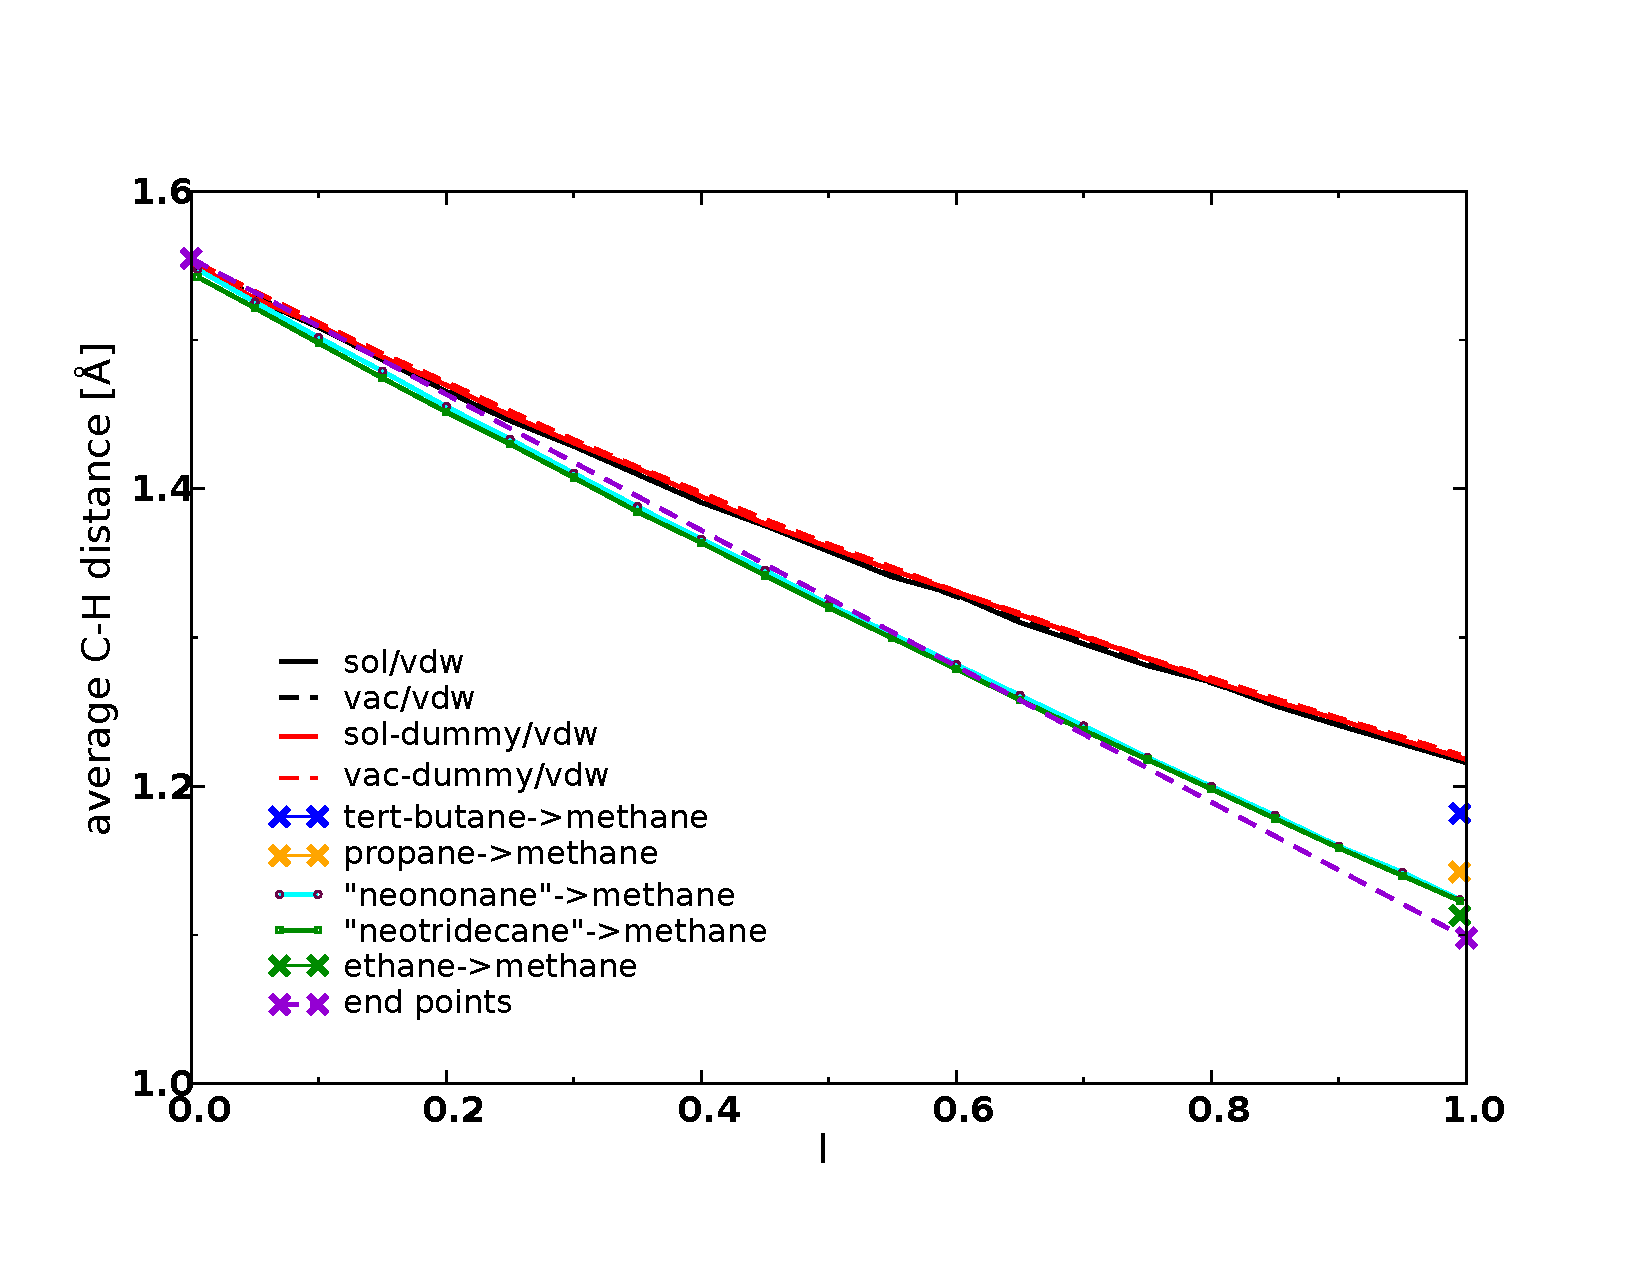
\includegraphics[scale=0.6]{figures/amber-dist.pdf}
\caption{The average C--H distance shown as a function of $\lambda$
  for the neopentane to methane and related cases.  The black and red
  lines display how the distance changes in solution and the
  vacuum phase, and with and without explicit dummy atoms.  The other test
  systems are designed to reduce the number of dummy atoms that
  surround the central carbon atom to show whether ``crowding'' is the
  cause of the issue.  The crosses denote end points only, in
  particular the violet crosses represent the non--perturbed end
  point distances.  For details see the text.}
\label{fig:amber-dist}
\end{figure}

The geometrical variation along $\lambda$ for the data in the main
text is shown in the black and red graphs.  The initial distance is
slightly smaller than what is expected from a C--H distance for the
particular atom types at $\lambda = 0$.  The final distance is about
\SI{1.23}{\angstrom} which is in contrast to the \SI{1.09}{\angstrom}
of the c3--hc bond of the GAFF force field.  The crosses in violet
mark the geometries of the ``pure'' (non--perturbed) end points and
are connected with a straight line.  The other crosses denote test
cases which successively replace the methyls on neopentane with
hydrogens.  The C--H distance decreases in correlation with the number
of the methyl groups i.e.\ tert-butane, propane, ethane.  This seems
to suggest that a ``crowding'' of dummy atoms around a central atom
compounds the problem of a too long C--H distance.  Neither of these
three test cases, however, displays the expected end point distance.

To further test this hypothesis methyl and ethyl groups are added to
all terminal methyl groups of neopentane, see cyan and green lines in
Figure~\ref{fig:amber-dist}.  In both cases the end point distance is
about \SI{1.12}{\angstrom} with a slightly lower value for the ethyl
substitution but which are still too high.

As Gromacs conveniently allows us to use a separate $\lambda$ for bonded
terms we tested this on the neopentane case.  After the charges were
transformed to the methane end state (dummy atoms have zero charges),
the bonded terms were mutated from neopentane to methane while the vdW
parameters were kept constant at the neopentane initial state.  The
observed end distance was about \SI{1.23}{\angstrom} which is to be
expected given that the symmetrically arranged methyl groups
will repel each other and thus not allow to reach the final distance.
Only after the final vdW (only) mutation had been carried out, were the final 
distances of \SI{1.09}{\angstrom} reached.

Table~\ref{tab:amber-disc} summarizes the free energy components for the 
2--methylindole to methane case for both forward and backward transformations.  
The electrostatic contributions display a very small SEM and the averages from 
both directions agree with each other up to the second digit after the comma.  
The van der Waals contributions show a higher SEM and the averages from the 
solution simulations agree well with each other.  However, the van der Waals 
contributions from the vacuum transformation are apart by 
\SI{0.3}{kcal.mol^{-1}} (highlighted in red).
\begin{table}
  \begin{minipage}{\linewidth}
    \caption{Free energy components for 2--methylindole computed from implicit dummy RAFE simulations.  The data are averages over three runs.}\label{tab:amber-disc}
    \makebox[\textwidth][c]{%
      \begin{tabular}{llrrrrrrrr}
        \toprule
        transformation & & $\Delta G_\mathrm{sol}^\mathrm{vdW}$ & SEM & $\Delta G_\mathrm{vac}^\mathrm{vdW}$  & SEM & $\Delta G_\mathrm{sol}^\mathrm{elec}$ & SEM & $\Delta G_\mathrm{vac}^\mathrm{elec}$ & SEM \\
        \midrule
2-methylindole  & methane      &  4.832 & 0.022 &  \hred{3.484} & 0.009 &  
19.419 & 0.007 &  11.989 & 0.001 \\
methane        & 2-methyindole & -4.900 & 0.017 & \hred{-3.185} & 0.011 & 
-19.412 & 0.009 & -11.989 & 0.001 \\
        \bottomrule
      \end{tabular}
    }
  \end{minipage}
\end{table}

In sum, this indicates a problem of the RAFE code in AMBER.  Whether that is a bug or a conceptual issue with the particular implementation can not be explained at the moment.

Table~\ref{tab:amber-5ring} summarizes the free energies obtained from forward 
and backward simulations of the cyclopentanyl transfer from position 2 to 
position 7 on indole and \emph{vice versa}.  Results from three different 
protocols are shown: 1) implicit dummy atoms and partial re/discharge of the 
5--ring only; 2) implicit dummy atoms and full re/discharge of all atoms; 3) 
explicit dummy atoms and partial re/discharge.  The free energies from the 
implicit dummy simulations agree very well with each other while the explicit 
dummy atom results are about \SI{0.2}{kcal.mol^{-1}} higher and forward and 
backward simulations have a larger hystersis of \SI{0.1}{kcal.mol^{-1}}.
\begin{table}
  \begin{minipage}{\linewidth}
    \caption{Free energies of hydration for the 2--cyclopentanylindole to 7--cyclopentanylindole case with three different protocols.  The data are averages over three runs.}\label{tab:amber-5ring}
    \makebox[\textwidth][c]{%
      \begin{tabular}{llrrrrrr}
        \toprule
        transformation & & $\Delta G_\mathrm{sol}$ & SEM & $\Delta G_\mathrm{vac}$ & SEM & $\Delta\Delta G_\mathrm{hydr} $ & SEM \\
        \midrule
implicit, partial & & & & & & \\
2--cyclopentanylindole & 7--cyclopentanylindole &  4.194 & 0.032 &  3.833 & 
0.014  &  0.361 & 0.032 \\
7--cyclopentanylindole & 2--cyclopentanylindole & -4.300 & 0.044 & -3.964 & 
0.011  & -0.335 & 0.045\\
\\
implicit, full & & & & & & \\
2--cyclopentanylindole & 7--cyclopentanylindole &  4.286 & 0.063 &  3.921 & 
0.028 &  0.365 & 0.069 \\
7--cyclopentanylindole & 2--cyclopentanylindole & -4.418 & 0.033 & -4.098 & 
0.014 & -0.320 & 0.036 \\
\\
explicit, partial & & & & & \\
2--cyclopentanylindole & 7--cyclopentanylindole &  4.145 & 0.041 &  3.517 & 
0.043 &  0.628 & 0.059 \\
7--cyclopentanylindole & 2--cyclopentanylindole & -4.256 & 0.030 & -3.759 & 
0.009 & -0.497 & 0.032 \\
        \bottomrule
      \end{tabular}
    }
  \end{minipage}
\end{table}


\subsection{Sire/SOMD}
\label{sec:sire-probs}


Figure ~\ref{fig:sire_histogram} compare relative free energy of hydration 
$\Delta\Delta G$ with relative $\Delta\Delta G$ estimations from absolute free  
energy calculations for all the transformation of dataset in 
~\ref{R-fig:cycles}.
%JM: Better to replace labels A-H with chemical structures?
%SB: I am afraid that substituting letters with chemical structures may result in a messy plot, but I will try
\begin{figure}[ht]
  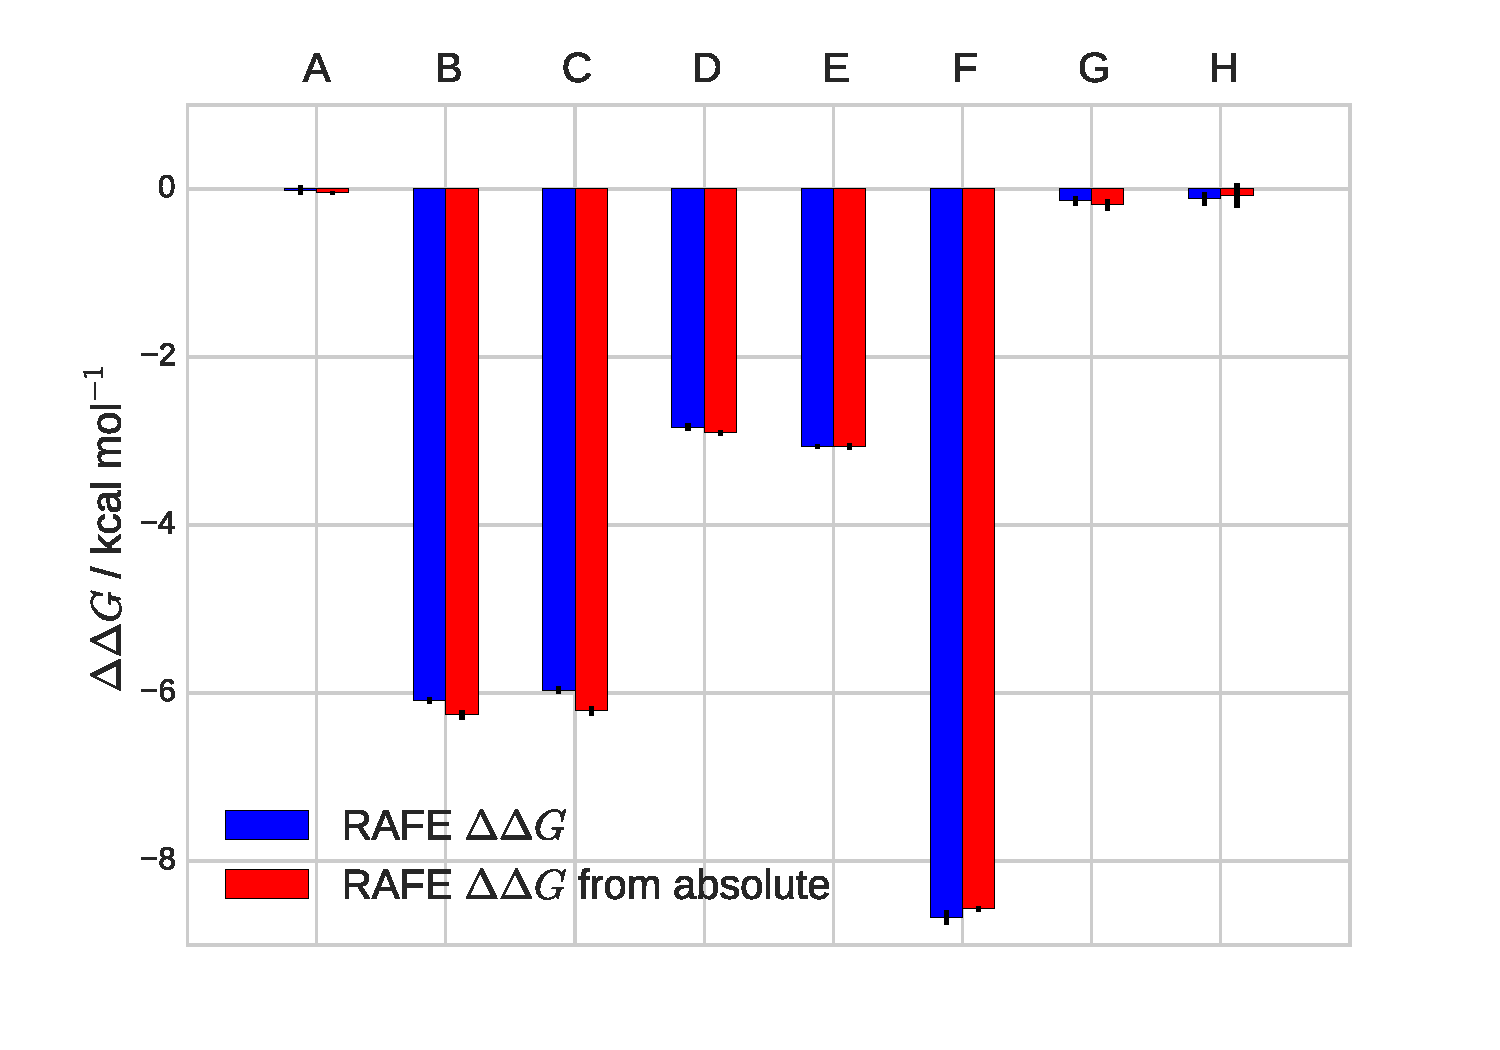
\includegraphics[width=\textwidth]{figures/sire_histogram.pdf}
  \caption{Relative free energy of hydration $\Delta\Delta G$, computed with 
  RAFE calculations, compared with $\Delta\Delta G$ derived from absolute free 
  energy calculations for A: methane to ethane, B: ethane to methanol, C: 
  methane to methanol, D: methane to 2-methylfuran, E: methane to toluene,
    F: methane to 2-methylindole, G: methane to neopentane, H: 
    2-cyclopentanylindole to 7-cyclopentanylindole.}
  \label{fig:sire_histogram}
\end{figure}


\begin{table}
  \begin{minipage}{\linewidth}
    \caption{Final relative free energy of hydration $\Delta\Delta G$ estimations and standard error SEM with Sire/SOMD unperturbed hydrogen bonds protocol, RAFE, compared with 
    relative free energy of hydration computed from absolute free energy simulations, RAFE-absolute. Signs in backward transformation are reverted for better comparison.}
    \label{tab:sire-finalresults}
    \makebox[\textwidth][c]{%
      \begin{tabular}{llrrrr}
        \toprule
         & & \multicolumn{2}{c}{RAFE} & \multicolumn{2}{c}{RAFE-absolute} \\
         transformation & &$\Delta\Delta G$ & SEM & $\Delta\Delta G$
         & SEM\\
        \midrule
ethane         & methane        & -0.01    & 0.05 & 0.04 & 0.02\\
methane        & ethane         & -0.04    & 0.02 & 0.04 & 0.02\\
methanol       & methane        &  5.99    & 0.05 & 6.21 & 0.05\\
methane        & methanol       &  5.96    & 0.04 & 6.21 & 0.05\\
ethane         & methanol       & -6.09    & 0.03 &-6.26 & 0.05\\
methanol       & ethane         & -6.09    & 0.02 &-6.26 & 0.05\\
toluene        & methane        &  2.89    & 0.03 & 3.06 & 0.03\\
methane        & toluene        &  3.06    & 0.02 & 3.06 & 0.03\\
neopentane\footnote{\label{foot:cent2}central mapping.} & methane &-0.20    & 
0.054 & -0.19 & 0.06\\
methane\footref{foot:cent2}        & neopentane     &-0.13   & 0.055 & -0.190  
& 0.060\\
neopentane\footnote{\label{foot:term2}terminal mapping.}    & methane        & 
-0.11   & 0.01 & -0.19 & 0.06\\
methane\footref{foot:term2}        & neopentane    &-0.10    & 0.06 &-0.19  
& 0.06\\
2-methylfuran  & methane        & 2.92    & 0.05 & 2.90  & 0.03\\
methane        & 2-methyfuran   & 2.83    & 0.03 & 2.90  & 0.03\\
2-methylindole & methane        & 8.64    & 0.06 & 8.57  & 0.03\\
methane        & 2-methylindole & 8.67    & 0.08 & 8.57  & 0.03\\
2--cyclopentanylindole & 7--cyclopentanylindole & 0.11 & 0.077 &  0.08 & 0.14\\
7--cyclopentanylindole & 2--cyclopentanylindole & 0.01 & 0.081 &  0.08 & 0.14 \\
	\bottomrule
      \end{tabular}
    }
  \end{minipage}
\end{table}

Table~\ref{tab:sire-finalresults} shows relative free energy of hydration 
$\Delta\Delta G$ compared to $\Delta\Delta G$ values extracted from absolute 
free energy calculations, depicted in Fig~\ref{fig:sire_histogram} in the paper.

Initially, Sire/SOMD RAFE protocols used all bonds constraint algorithm. In this way all the solute bonds are constrained, which results in a
systematic offset for each RAFE predictions, compared to the RAFE from absolute free energy calculations.
Figure ~\ref{fig:sire_allbonds} show the discrepancy between RAFE computed with all bond constraints and RAFE from absolute free energy calculations.


\begin{figure}[ht]
  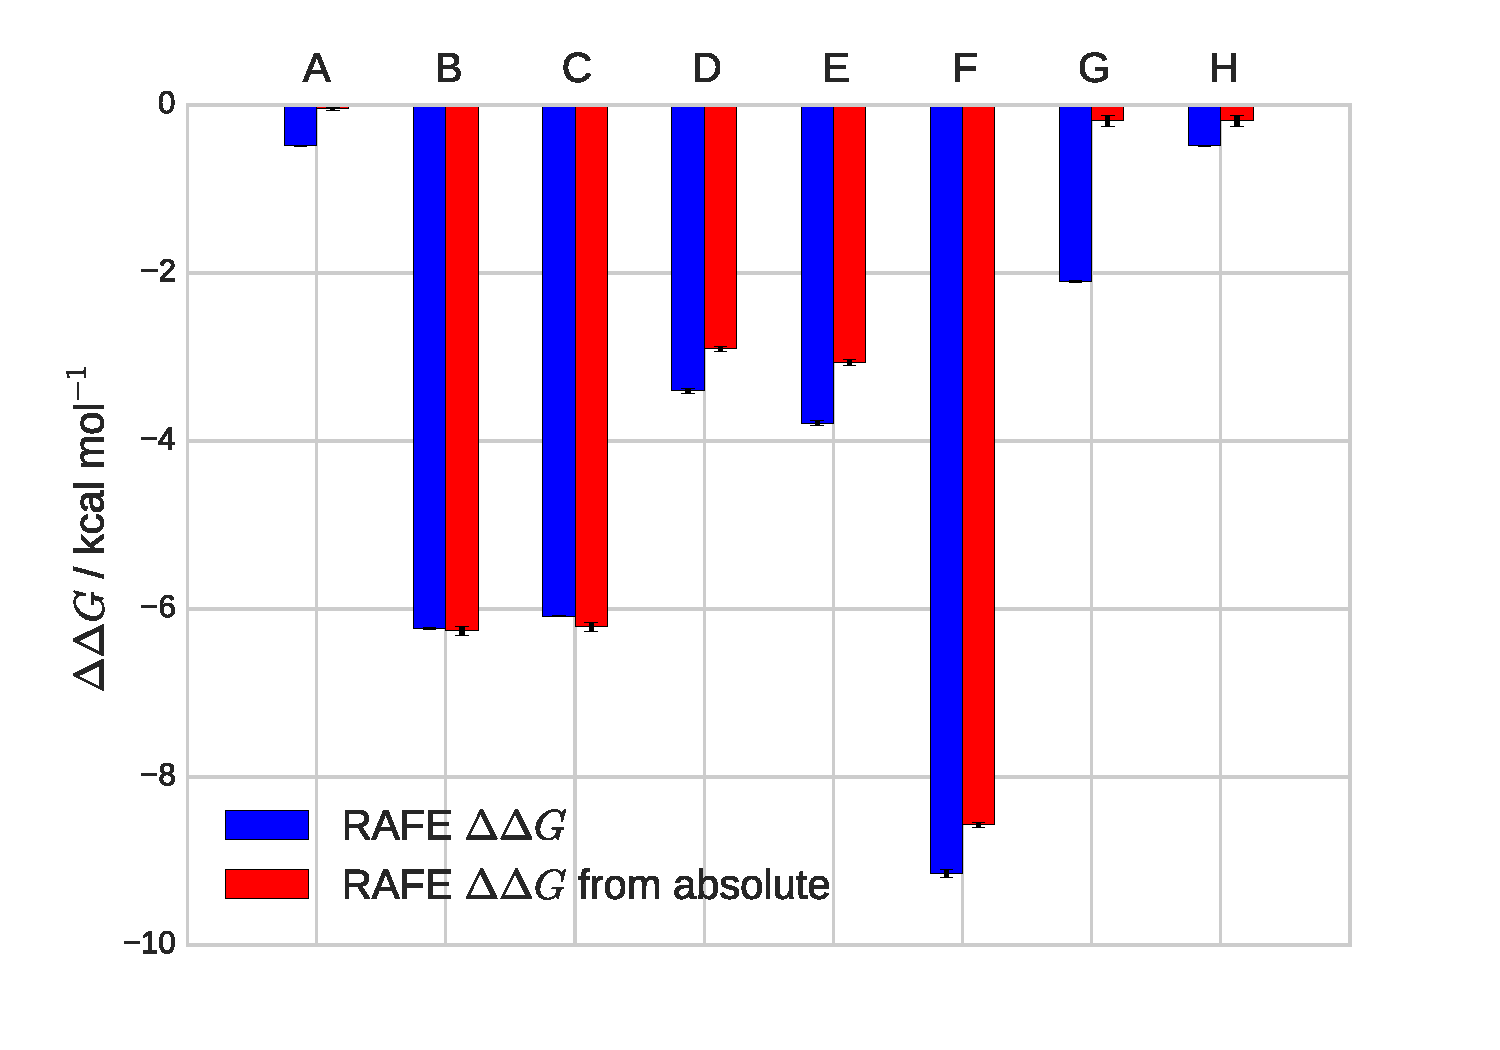
\includegraphics[width=\textwidth]{figures/SI_sire_allbonds_relabs.pdf}
  \caption{Comparison between RAFE of hydration computed with all bond constraints and RAFE computed from absolute free energy calculations}
  \label{fig:sire_allbonds}
\end{figure}

Finally, figure~\ref{fig:sire_constraints} and tab.~\ref{tab:sire_constraints} compare relative free energy of hydration $\Delta \Delta G$ estimated with RAFE using all bonds constraints, no constraints and unperturbed hydrogen bond constraints.

\begin{figure}[ht]
  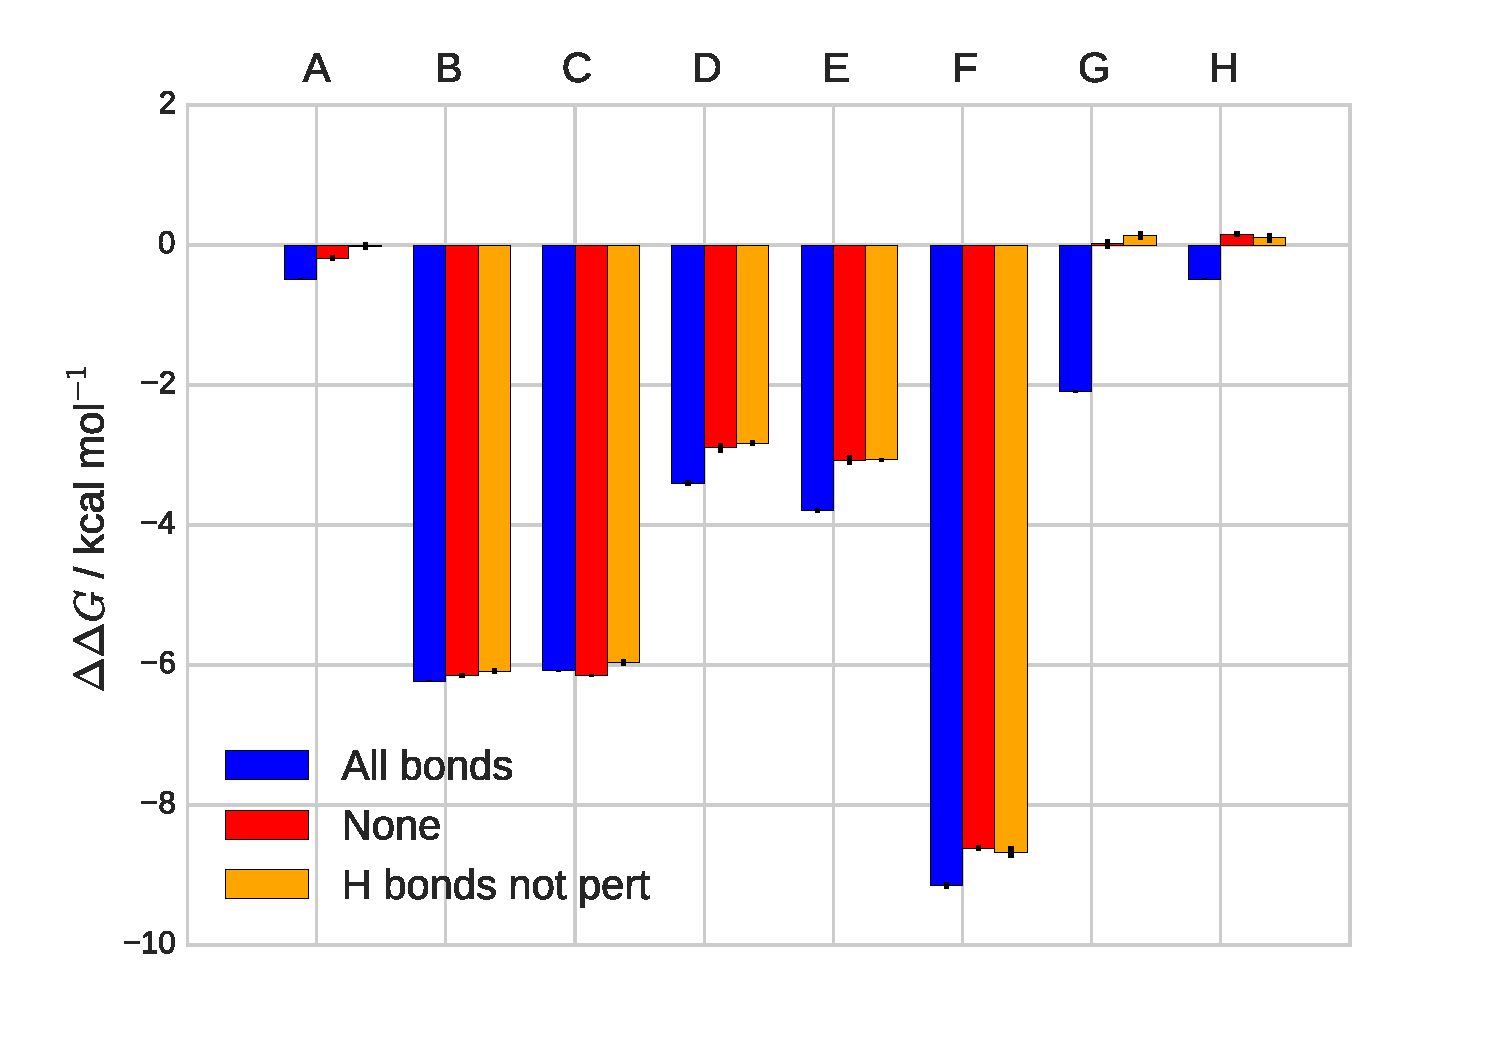
\includegraphics[width=\textwidth]{figures/SI_sire_constraints.pdf}
  \caption{Comparison between RAFE of hydration computed with all bond constraints, no constraints and unperturbed hydrogen bonds constraint}
  \label{fig:sire_constraints}
\end{figure}

\begin{table}
  \begin{minipage}{\linewidth}
    \caption{Relative free energy of hydration $\Delta\Delta G$ computed with all bond constraints, \textit{All bonds}, no constraints, \textit{None}, and unperturbed hydrogen bond constraint, \textit{unpert H bonds} }
    \label{tab:sire_constraints}
    \makebox[\textwidth][c]{%
      \begin{tabular}{llrrrrrr}
        \toprule
         & & \multicolumn{2}{c}{All bonds} & \multicolumn{2}{c}{None} & 
         \multicolumn{2}{c}{unpert H bonds} \\
         transformation &  &$\Delta\Delta G$ & SEM & $\Delta\Delta G$ & SEM & $\Delta\Delta G$ & SEM \\
        \midrule
ethane         & methane        &-0.48 & 0.01 &-0.18 & 0.04 & -0.01 & 0.05\\
methane        & ethane         &-0.49 & 0.01 &-0.01 & 0.02 & -0.04 & 0.02\\ 
methanol       & methane        & 6.06 & 0.01 & 6.49 & 0.01 &  5.99 & 0.05\\
methane        & methanol       & 6.08 & 0.01 & 6.15 & 0.01 &  5.96 & 0.04\\
ethane         & methanol       &-6.22 & 0.01 &-6.14 & 0.03 & -6.09 & 0.03\\
methanol       & ethane         &-6.23 & 0.01 &-6.09 & 0.01 & -6.09 & 0.02\\
toluene        & methane        & 3.73 & 0.27 & 3.09 & 0.06 &  2.89 & 0.09\\
methane        & toluene        & 3.79 & 0.03 & 3.07 & 0.06 &  3.06 & 0.02\\
neopentane\footnote{\label{foot:cent3}central mapping.} & methane  &-2.09 & 
0.01 &-0.14 & 0.14   &-0.20    & 0.05\\
methane\footref{foot:cent3}        & neopentane     &-2.04 & 0.01 &-0.018 & 
0.06  &-0.13   & 0.05\\
neopentane\footnote{\label{foot:term3}terminal mapping.}    & methane  &-0.48
& 0.01  &-0.14 & 0.06 & -0.11   & 0.01\\
methane\footref{foot:term3}        & neopentane    &-0.59 & 0.02  &-0.14 & 
0.060   &-0.10   & 0.06\\
2-methylfuran  & methane        & 3.38 & 0.02 & 2.81 & 0.03 & 2.92  & 0.05\\
methane        & 2-methyfuran   & 3.40 & 0.03 & 2.89 & 0.06 & 2.83  & 0.03\\
2-methylindole & methane        & 9.29 & 0.06 & 8.72 & 0.05 & 8.63  & 0.06\\
methane        & 2-methylindole & 9.10 & 0.04 & 8.61 & 0.04 & 8.67  & 0.08\\
	\bottomrule
      \end{tabular}
    }
  \end{minipage}
\end{table}

\subsection{GROMACS}
\label{sec:gromacs-probs}

Table~\ref{tab:gro-sc2} compares RAFE results subject to the use of Coulomb softcore potentials.
In principle, the use of softcore functions is redundant in the split protocol because charges are
changed while van der Waals parameters are fully tuned to the transformation's final state parameters.
SEM values tend to be larger when they are used.

\begin{table}[]
  \begin{minipage}{\linewidth}
  \caption{$\Delta \Delta G_{hydr}$ results in different scenarios with or without Coulomb softcore potentials, in kcal $\cdot$ mol$^{-1}$.}
  \label{tab:gro-sc2}
  \resizebox{\columnwidth}{!}{%
  \begin{tabular}{@{}llllllll@{}}
    \toprule
     &  & \multicolumn{2}{l}{without Coulomb softcore} & \multicolumn{2}{l}{with Coulomb softcore} & \multicolumn{2}{l}{absolute} \\
     &  & RF & PME & RF & PME & RF & PME \\
    \multicolumn{2}{l}{Transformations} & $\Delta \Delta G$ & $\Delta \Delta G$ & $\Delta \Delta G$ & $\Delta \Delta G$ & $\Delta \Delta G$ & $\Delta \Delta G$ \\ \midrule
    ethane & methane & \num{-0.025 +- 0.005} & \num{-0.035 +- 0.02} & \num{-0.03+-0.04} & \num{-0.02+-0.04} & \num{-0.06 +- 0.01} & \num{-0.04 +- 0.01} \\
    methane & ethane & \num{-0.01 +- 0.02} & \num{-0.02 +- 0.01} & \num{-0.01+-0.04} & \num{-0.02+-0.04} &  &  \\
    methanol & methane & \num{6.163 +- 0.006} & \num{6.197 +- 0.004} & \num{7.32+-0.03} & \num{7.42+-0.04} & \num{5.77 +- 0.01} & \num{5.95 +- 0.01} \\
    methane & methanol & \num{6.168 +- 0.005} & \num{6.199 +- 0.008} & \num{7.14+-0.03} & \num{7.21+-0.03} &  &  \\
    ethane & methanol & \num{-6.123 +- 0.007} & \num{-6.185 +- 0.006} & 
    \num{-6.15+-0.02} & \num{-6.21+-0.02} & \num{-5.83 +- 0.01} & \num{-5.98 +- 
    0.01} \\
    methanol & ethane & \num{-6.124 +- 0.005} & \num{-6.193+- 0.004} & \num{-6.15+-0.02} & \num{-6.21+-0.02} &  &  \\
    toluene & methane & \num{3.22 +- 0.01} & \num{3.211 +- 0.006} & \num{3.22+-0.04} & \num{3.21+-0.04} & \num{2.97 +- 0.01} & \num{3.16 +- 0.01} \\
    methane & toluene & \num{3.25 +- 0.01} & \num{3.20 +- 0.01} & \num{3.27+-0.04} & \num{3.22+-0.04} &  &  \\
    neopentane\footnote{\label{foot:c-map}central mapping} & methane & 
    \num{-0.103 +- 0.008} & \num{-0.15 +- 0.02} & \num{-0.13+-0.08} & 
    \num{-0.13+-0.08} & \num{-0.18 +- 0.01} & \num{-0.14 +- 0.01} \\
    methane\footref{foot:c-map} & neopentane & \num{-0.11 +- 0.02} & \num{-0.16 
    +- 0.05} & \num{-0.12+-0.08} & \num{-0.15+-0.08} &  &  \\
    neopentane\footnote{\label{foot:t-map}terminal mapping} & methane & 
    \num{-0.116 +- 0.007} & \num{-0.13 +- 0.01} & \num{-0.10+-0.04} & 
    \num{-0.13+-0.04} &  &  \\
    methane\footref{foot:t-map} & neopentane2 & \num{-0.10 +- 0.03} & 
    \num{-0.18 +- 0.03} & \num{-0.08+-0.06} & \num{0.15+-0.06} &  &  \\
    2-methylfuran & methane & \num{2.986 +- 0.006} & \num{2.930 +- 0.05} & \num{3.07+-0.03} & \num{3.02+-0.04} & \num{2.87 +- 0.01} & \num{2.95 +- 0.01} \\
    methane & 2-methylfuran & \num{3.007 +- 0.004} & \num{2.96 +- 0.01} & \num{3.08+-0.03} & \num{3.02+-0.04} &  &  \\
    2-methylindole & methane & \num{8.71 +- 0.02} & \num{8.73 +- 0.03} & \num{8.79+-0.04} & \num{8.82+-0.05} & \num{8.44 +- 0.02} & \num{8.79 +- 0.02} \\
    methane & 2-methylindole & \num{8.73 +- 0.03} & \num{8.74 +- 0.01} & \num{8.79+-0.05} & \num{8.81+-0.06} &  &  \\
    2-cyclopentanylindole & 7-cyclopentanylindole & \num{-0.07 +- 0.02} & \num{-0.03 +- 0.03} & \num{-0.12+-0.03} & \num{-0.14+-0.05} & \num{-0.02 +- 0.05} & \num{0.02 +- 0.02} \\
    7-cyclopentanylindole & 2-cyclopentanylindole & \num{-0.12 +- 0.06} & 
    \num{-0.20 +- 0.04} & \num{1.2+-0.2}\footnote{\label{foot:inv} inverted 
    sign} & \num{1.5+-0.1}\footref{foot:inv} &  &  \\ \bottomrule
  \end{tabular}}
\end{minipage}
\end{table}

The effect of the Coulomb softcore potential can be seen in Figure \ref{fig:gro_sc_eff}. 

\begin{figure}[ht]
  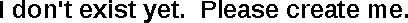
\includegraphics{figures/TI_plot.pdf}
  \caption{$\langle\partial\mathscr{H}/\partial\lambda\rangle$ plot for the 
  change in electrostatic terms in methane $\rightarrow$ methanol.}
  \label{fig:gro_sc_eff}
\end{figure}

\bibliography{journal-abbrev,reprod}

\end{document}
